% Editable textbook TikZ, initially imported from the verified semantic plate.
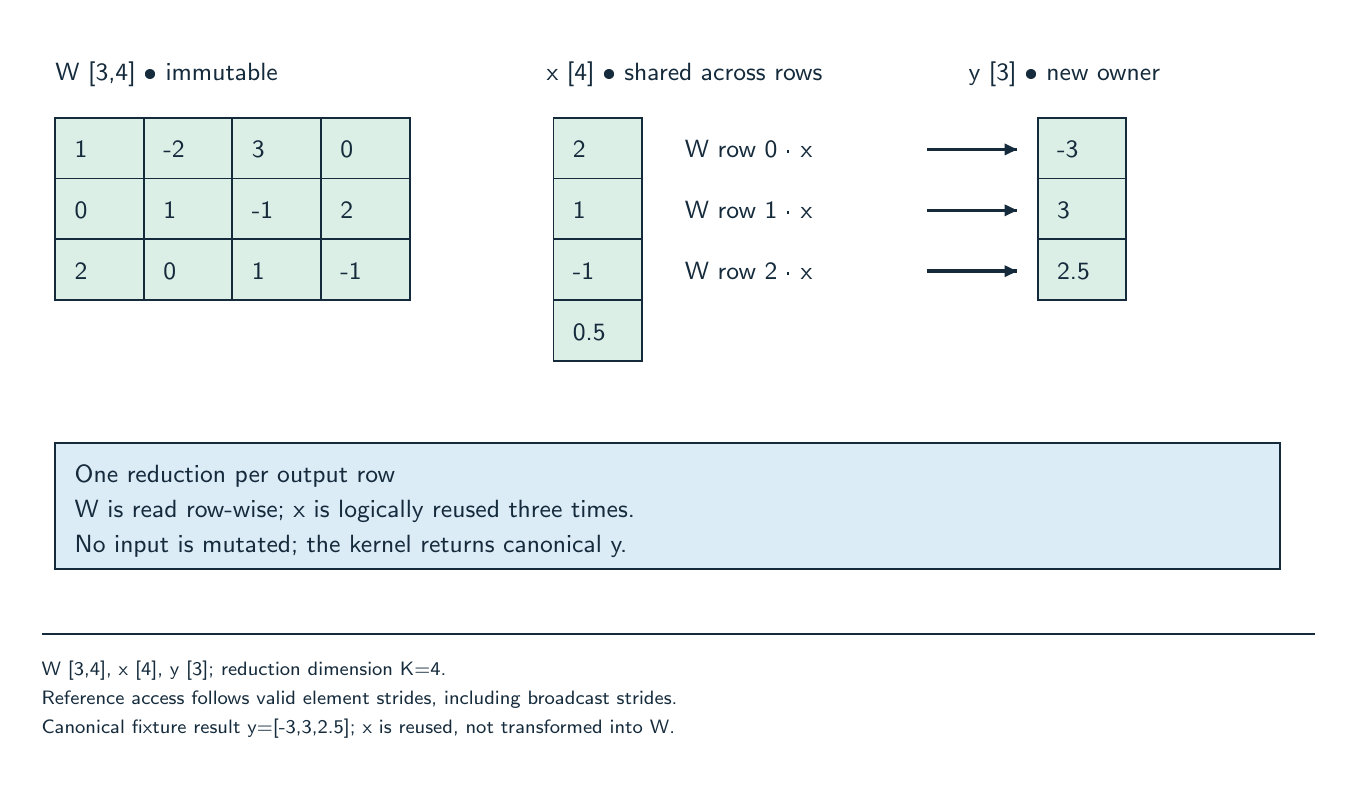
\begin{tikzpicture}[x=.5pt,y=-.5pt]
\path[use as bounding box] (30,170) rectangle (975,700);
\node[inner sep=0pt,outer sep=0pt,anchor=base west,text={rgb,255:red,21;green,43;blue,60},font=\sffamily\fontsize{9.5}{11.4}\selectfont] at (50,208) {W [3,4] • immutable};
\path[fill={rgb,255:red,220;green,239;blue,231},draw={rgb,255:red,21;green,43;blue,60},line width=0.7pt] (50.0,235.0) rectangle (114.0,279.0);
\node[inner sep=0pt,outer sep=0pt,anchor=base west,text={rgb,255:red,21;green,43;blue,60},font=\sffamily\fontsize{9.0}{10.799999999999999}\selectfont] at (64,264) {1};
\path[fill={rgb,255:red,220;green,239;blue,231},draw={rgb,255:red,21;green,43;blue,60},line width=0.7pt] (114.0,235.0) rectangle (178.0,279.0);
\node[inner sep=0pt,outer sep=0pt,anchor=base west,text={rgb,255:red,21;green,43;blue,60},font=\sffamily\fontsize{9.0}{10.799999999999999}\selectfont] at (128,264) {-2};
\path[fill={rgb,255:red,220;green,239;blue,231},draw={rgb,255:red,21;green,43;blue,60},line width=0.7pt] (178.0,235.0) rectangle (242.0,279.0);
\node[inner sep=0pt,outer sep=0pt,anchor=base west,text={rgb,255:red,21;green,43;blue,60},font=\sffamily\fontsize{9.0}{10.799999999999999}\selectfont] at (192,264) {3};
\path[fill={rgb,255:red,220;green,239;blue,231},draw={rgb,255:red,21;green,43;blue,60},line width=0.7pt] (242.0,235.0) rectangle (306.0,279.0);
\node[inner sep=0pt,outer sep=0pt,anchor=base west,text={rgb,255:red,21;green,43;blue,60},font=\sffamily\fontsize{9.0}{10.799999999999999}\selectfont] at (256,264) {0};
\path[fill={rgb,255:red,220;green,239;blue,231},draw={rgb,255:red,21;green,43;blue,60},line width=0.7pt] (50.0,279.0) rectangle (114.0,323.0);
\node[inner sep=0pt,outer sep=0pt,anchor=base west,text={rgb,255:red,21;green,43;blue,60},font=\sffamily\fontsize{9.0}{10.799999999999999}\selectfont] at (64,308) {0};
\path[fill={rgb,255:red,220;green,239;blue,231},draw={rgb,255:red,21;green,43;blue,60},line width=0.7pt] (114.0,279.0) rectangle (178.0,323.0);
\node[inner sep=0pt,outer sep=0pt,anchor=base west,text={rgb,255:red,21;green,43;blue,60},font=\sffamily\fontsize{9.0}{10.799999999999999}\selectfont] at (128,308) {1};
\path[fill={rgb,255:red,220;green,239;blue,231},draw={rgb,255:red,21;green,43;blue,60},line width=0.7pt] (178.0,279.0) rectangle (242.0,323.0);
\node[inner sep=0pt,outer sep=0pt,anchor=base west,text={rgb,255:red,21;green,43;blue,60},font=\sffamily\fontsize{9.0}{10.799999999999999}\selectfont] at (192,308) {-1};
\path[fill={rgb,255:red,220;green,239;blue,231},draw={rgb,255:red,21;green,43;blue,60},line width=0.7pt] (242.0,279.0) rectangle (306.0,323.0);
\node[inner sep=0pt,outer sep=0pt,anchor=base west,text={rgb,255:red,21;green,43;blue,60},font=\sffamily\fontsize{9.0}{10.799999999999999}\selectfont] at (256,308) {2};
\path[fill={rgb,255:red,220;green,239;blue,231},draw={rgb,255:red,21;green,43;blue,60},line width=0.7pt] (50.0,323.0) rectangle (114.0,367.0);
\node[inner sep=0pt,outer sep=0pt,anchor=base west,text={rgb,255:red,21;green,43;blue,60},font=\sffamily\fontsize{9.0}{10.799999999999999}\selectfont] at (64,352) {2};
\path[fill={rgb,255:red,220;green,239;blue,231},draw={rgb,255:red,21;green,43;blue,60},line width=0.7pt] (114.0,323.0) rectangle (178.0,367.0);
\node[inner sep=0pt,outer sep=0pt,anchor=base west,text={rgb,255:red,21;green,43;blue,60},font=\sffamily\fontsize{9.0}{10.799999999999999}\selectfont] at (128,352) {0};
\path[fill={rgb,255:red,220;green,239;blue,231},draw={rgb,255:red,21;green,43;blue,60},line width=0.7pt] (178.0,323.0) rectangle (242.0,367.0);
\node[inner sep=0pt,outer sep=0pt,anchor=base west,text={rgb,255:red,21;green,43;blue,60},font=\sffamily\fontsize{9.0}{10.799999999999999}\selectfont] at (192,352) {1};
\path[fill={rgb,255:red,220;green,239;blue,231},draw={rgb,255:red,21;green,43;blue,60},line width=0.7pt] (242.0,323.0) rectangle (306.0,367.0);
\node[inner sep=0pt,outer sep=0pt,anchor=base west,text={rgb,255:red,21;green,43;blue,60},font=\sffamily\fontsize{9.0}{10.799999999999999}\selectfont] at (256,352) {-1};
\node[inner sep=0pt,outer sep=0pt,anchor=base west,text={rgb,255:red,21;green,43;blue,60},font=\sffamily\fontsize{9.5}{11.4}\selectfont] at (405,208) {x [4] • shared across rows};
\path[fill={rgb,255:red,220;green,239;blue,231},draw={rgb,255:red,21;green,43;blue,60},line width=0.7pt] (410.0,235.0) rectangle (474.0,279.0);
\node[inner sep=0pt,outer sep=0pt,anchor=base west,text={rgb,255:red,21;green,43;blue,60},font=\sffamily\fontsize{9.0}{10.799999999999999}\selectfont] at (424,264) {2};
\path[fill={rgb,255:red,220;green,239;blue,231},draw={rgb,255:red,21;green,43;blue,60},line width=0.7pt] (410.0,279.0) rectangle (474.0,323.0);
\node[inner sep=0pt,outer sep=0pt,anchor=base west,text={rgb,255:red,21;green,43;blue,60},font=\sffamily\fontsize{9.0}{10.799999999999999}\selectfont] at (424,308) {1};
\path[fill={rgb,255:red,220;green,239;blue,231},draw={rgb,255:red,21;green,43;blue,60},line width=0.7pt] (410.0,323.0) rectangle (474.0,367.0);
\node[inner sep=0pt,outer sep=0pt,anchor=base west,text={rgb,255:red,21;green,43;blue,60},font=\sffamily\fontsize{9.0}{10.799999999999999}\selectfont] at (424,352) {-1};
\path[fill={rgb,255:red,220;green,239;blue,231},draw={rgb,255:red,21;green,43;blue,60},line width=0.7pt] (410.0,367.0) rectangle (474.0,411.0);
\node[inner sep=0pt,outer sep=0pt,anchor=base west,text={rgb,255:red,21;green,43;blue,60},font=\sffamily\fontsize{9.0}{10.799999999999999}\selectfont] at (424,396) {0.5};
\node[inner sep=0pt,outer sep=0pt,anchor=base west,text={rgb,255:red,21;green,43;blue,60},font=\sffamily\fontsize{9.5}{11.4}\selectfont] at (710,208) {y [3] • new owner};
\path[fill={rgb,255:red,220;green,239;blue,231},draw={rgb,255:red,21;green,43;blue,60},line width=0.7pt] (760.0,235.0) rectangle (824.0,279.0);
\node[inner sep=0pt,outer sep=0pt,anchor=base west,text={rgb,255:red,21;green,43;blue,60},font=\sffamily\fontsize{9.0}{10.799999999999999}\selectfont] at (774,264) {-3};
\path[fill={rgb,255:red,220;green,239;blue,231},draw={rgb,255:red,21;green,43;blue,60},line width=0.7pt] (760.0,279.0) rectangle (824.0,323.0);
\node[inner sep=0pt,outer sep=0pt,anchor=base west,text={rgb,255:red,21;green,43;blue,60},font=\sffamily\fontsize{9.0}{10.799999999999999}\selectfont] at (774,308) {3};
\path[fill={rgb,255:red,220;green,239;blue,231},draw={rgb,255:red,21;green,43;blue,60},line width=0.7pt] (760.0,323.0) rectangle (824.0,367.0);
\node[inner sep=0pt,outer sep=0pt,anchor=base west,text={rgb,255:red,21;green,43;blue,60},font=\sffamily\fontsize{9.0}{10.799999999999999}\selectfont] at (774,352) {2.5};
\node[inner sep=0pt,outer sep=0pt,anchor=base west,text={rgb,255:red,21;green,43;blue,60},font=\sffamily\fontsize{9.0}{10.799999999999999}\selectfont] at (505,264) {W row 0 · x};
\draw[fill=none,draw={rgb,255:red,21;green,43;blue,60},line width=1.25pt] (680,258) -- (745,258);
\path[fill={rgb,255:red,21;green,43;blue,60},draw=none,line width=0.5pt] (745.00,258.00) -- (736.00,262.35) -- (736.00,253.65) -- cycle;
\node[inner sep=0pt,outer sep=0pt,anchor=base west,text={rgb,255:red,21;green,43;blue,60},font=\sffamily\fontsize{9.0}{10.799999999999999}\selectfont] at (505,308) {W row 1 · x};
\draw[fill=none,draw={rgb,255:red,21;green,43;blue,60},line width=1.25pt] (680,302) -- (745,302);
\path[fill={rgb,255:red,21;green,43;blue,60},draw=none,line width=0.5pt] (745.00,302.00) -- (736.00,306.35) -- (736.00,297.65) -- cycle;
\node[inner sep=0pt,outer sep=0pt,anchor=base west,text={rgb,255:red,21;green,43;blue,60},font=\sffamily\fontsize{9.0}{10.799999999999999}\selectfont] at (505,352) {W row 2 · x};
\draw[fill=none,draw={rgb,255:red,21;green,43;blue,60},line width=1.25pt] (680,346) -- (745,346);
\path[fill={rgb,255:red,21;green,43;blue,60},draw=none,line width=0.5pt] (745.00,346.00) -- (736.00,350.35) -- (736.00,341.65) -- cycle;
\path[fill={rgb,255:red,220;green,236;blue,247},draw={rgb,255:red,21;green,43;blue,60},line width=0.7pt] (50.0,470.0) rectangle (935.0,561.0);
\node[inner sep=0pt,outer sep=0pt,anchor=base west,text={rgb,255:red,21;green,43;blue,60},font=\sffamily\fontsize{9.0}{10.799999999999999}\selectfont] at (64,499) {One reduction per output row};
\node[inner sep=0pt,outer sep=0pt,anchor=base west,text={rgb,255:red,21;green,43;blue,60},font=\sffamily\fontsize{9.0}{10.799999999999999}\selectfont] at (64,524) {W is read row-wise; x is logically reused three times.};
\node[inner sep=0pt,outer sep=0pt,anchor=base west,text={rgb,255:red,21;green,43;blue,60},font=\sffamily\fontsize{9.0}{10.799999999999999}\selectfont] at (64,549) {No input is mutated; the kernel returns canonical y.};
\draw[fill=none,draw={rgb,255:red,21;green,43;blue,60},line width=0.75pt] (40,608) -- (960,608);
\node[inner sep=0pt,outer sep=0pt,anchor=base west,text={rgb,255:red,21;green,43;blue,60},font=\sffamily\fontsize{7.5}{9.0}\selectfont] at (40,638) {W [3,4], x [4], y [3]; reduction dimension K=4.};
\node[inner sep=0pt,outer sep=0pt,anchor=base west,text={rgb,255:red,21;green,43;blue,60},font=\sffamily\fontsize{7.5}{9.0}\selectfont] at (40,659) {Reference access follows valid element strides, including broadcast strides.};
\node[inner sep=0pt,outer sep=0pt,anchor=base west,text={rgb,255:red,21;green,43;blue,60},font=\sffamily\fontsize{7.5}{9.0}\selectfont] at (40,680) {Canonical fixture result y=[-3,3,2.5]; x is reused, not transformed into W.};
\end{tikzpicture}
